%%
%% Copyright Guy Taylor 2012
%%
%%
\chapter{Code Analysis}

\begin{figure}[htb]
  \centering
  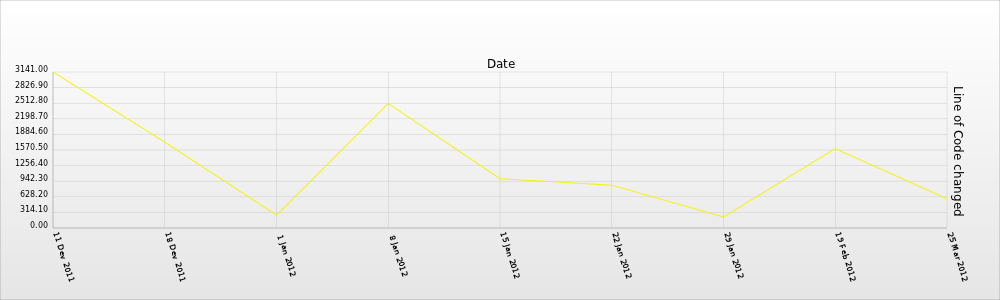
\includegraphics[width=\textwidth, keepaspectratio=true]{images/git_work_time.png}
  \caption{Work over time}
  \label{fig:git_work_time}
\end{figure}

To generate Figure \ref{fig:git_work_time} I utilised the \url{http://www.GitHub.com} ``Impact'' graphic.
The values from this graphic where subsequently amended to take account of commit
\texttt{ee91d95da7ed2e4d4779b48c7487ad86d37a1fb1} and
\texttt{1701925f0a310ea00a195e64fc0379ab963e1cf3} as these they contained a unproportional
amount of code not produced by myself.

%
%created gcc version
%  ee91d95da7ed2e4d4779b48c7487ad86d37a1fb1
%  07-01-2012
%
%created the GDB proxy
%  d9aaa51e7ff5d0ed034394ca24cd5bb5e0094761
%  07-01-2012
%
%created the debug module:
%  c198234eb5e72eaa36718fe5923b2c190acd5d12
%  09-01-2012
%
%created the newlib module
%  7ff54e992224314404a202c366fcea095687a163
%  17-01-2012
%
%created the radio module
%  7ff54e992224314404a202c366fcea095687a163
%  17-01-2012
%
